% Options for packages loaded elsewhere
\PassOptionsToPackage{unicode}{hyperref}
\PassOptionsToPackage{hyphens}{url}
%
\documentclass[
]{article}
\usepackage{amsmath,amssymb}
\usepackage{lmodern}
\usepackage{iftex}
\ifPDFTeX
  \usepackage[T1]{fontenc}
  \usepackage[utf8]{inputenc}
  \usepackage{textcomp} % provide euro and other symbols
\else % if luatex or xetex
  \usepackage{unicode-math}
  \defaultfontfeatures{Scale=MatchLowercase}
  \defaultfontfeatures[\rmfamily]{Ligatures=TeX,Scale=1}
\fi
% Use upquote if available, for straight quotes in verbatim environments
\IfFileExists{upquote.sty}{\usepackage{upquote}}{}
\IfFileExists{microtype.sty}{% use microtype if available
  \usepackage[]{microtype}
  \UseMicrotypeSet[protrusion]{basicmath} % disable protrusion for tt fonts
}{}
\makeatletter
\@ifundefined{KOMAClassName}{% if non-KOMA class
  \IfFileExists{parskip.sty}{%
    \usepackage{parskip}
  }{% else
    \setlength{\parindent}{0pt}
    \setlength{\parskip}{6pt plus 2pt minus 1pt}}
}{% if KOMA class
  \KOMAoptions{parskip=half}}
\makeatother
\usepackage{xcolor}
\usepackage[margin=1in]{geometry}
\usepackage{longtable,booktabs,array}
\usepackage{calc} % for calculating minipage widths
% Correct order of tables after \paragraph or \subparagraph
\usepackage{etoolbox}
\makeatletter
\patchcmd\longtable{\par}{\if@noskipsec\mbox{}\fi\par}{}{}
\makeatother
% Allow footnotes in longtable head/foot
\IfFileExists{footnotehyper.sty}{\usepackage{footnotehyper}}{\usepackage{footnote}}
\makesavenoteenv{longtable}
\usepackage{graphicx}
\makeatletter
\def\maxwidth{\ifdim\Gin@nat@width>\linewidth\linewidth\else\Gin@nat@width\fi}
\def\maxheight{\ifdim\Gin@nat@height>\textheight\textheight\else\Gin@nat@height\fi}
\makeatother
% Scale images if necessary, so that they will not overflow the page
% margins by default, and it is still possible to overwrite the defaults
% using explicit options in \includegraphics[width, height, ...]{}
\setkeys{Gin}{width=\maxwidth,height=\maxheight,keepaspectratio}
% Set default figure placement to htbp
\makeatletter
\def\fps@figure{htbp}
\makeatother
\setlength{\emergencystretch}{3em} % prevent overfull lines
\providecommand{\tightlist}{%
  \setlength{\itemsep}{0pt}\setlength{\parskip}{0pt}}
\setcounter{secnumdepth}{-\maxdimen} % remove section numbering
\ifLuaTeX
  \usepackage{selnolig}  % disable illegal ligatures
\fi
\IfFileExists{bookmark.sty}{\usepackage{bookmark}}{\usepackage{hyperref}}
\IfFileExists{xurl.sty}{\usepackage{xurl}}{} % add URL line breaks if available
\urlstyle{same} % disable monospaced font for URLs
\hypersetup{
  hidelinks,
  pdfcreator={LaTeX via pandoc}}

\author{}
\date{\vspace{-2.5em}}

\begin{document}

\begin{longtable}[]{@{}l@{}}
\toprule()
\textbackslash begin\{document\} \\
\midrule()
\endhead
title: ``Proteome wide screen for RNA-dependent Proteins in interphasic
HeLa cells'' \\
author: ``Bolz, C., Bonsen, M., Pott, M., Simon, M.'' \\
date: ``2022-07-16'' \\
output: \\
pdf\_document: default \\
html\_document: default \\
df\_print: paged \\
\bottomrule()
\end{longtable}

\hypertarget{introduction}{%
\section{Introduction}\label{introduction}}

RNA and proteins represent a symbiotic system. Proteins need RNA as a
template for their biosynthesis as stated by Francis Crick in his
``Central Dogma of Molecular Biology'' (Crick, 1970). Vice versa,
studies have shown that proteins need RNA for their catalytic activity,
for instance in the RNA-induced silencing complex (Pratt and Macrae,
2009; Wilson and Doudna, 2013). Additionally, some RNA depends on
proteins for its synthesis and stability (Kishore \emph{et al.}, 2010).
A family of proteins which illustrates this symbiotic relationship are
RNA-binding proteins (RBPs). RBPs present a class of proteins whose
interactome depends on RNA. They were shown to play a crucial role in
RNA metabolism (Kishore \emph{et al.}, 2010), cancer development (Wei
\emph{et al.}, 2022), and genetic disease (Gebauer \emph{et al.}, 2021).
Therefore, a deeper understanding of RNA binding and RNA-Protein
interaction strengthens our ability to adjust and modulate the cellular
mechanisms affected.

RBPs can be further categorized into ``true'' RBPs (e.g.~DICER, NPM3),
those RNA-binding proteins which directly bind to RNA, and ``RBP
interacting proteins'' which merely interact with ``true'' RBPs (eg.
RBBP7). Furthermore, ``true'' RBPs can be subcategorized into
``RNA-dependent'', meaning relying on RNA for their whole and correct
function (eg. DICER) and ``partially RNA dependent'', those that only
require RNA for certain functions or transport (eg. NPM3) (see Fig. 1)
(Caudron-Herger \emph{et al.}, 2019; Corley \emph{et al.}, 2020).

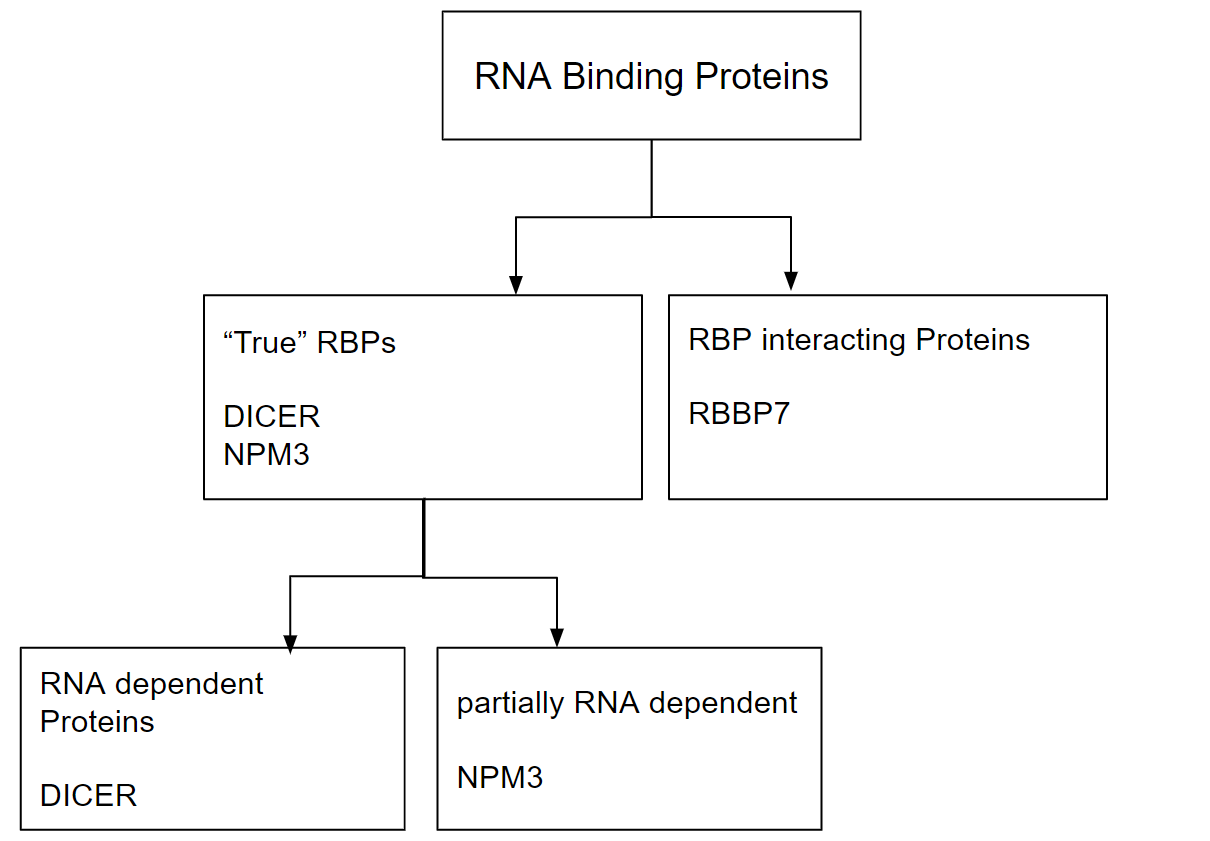
\includegraphics{../../Figure1.PNG}

\textbf{Figure 1}. Categorization of RNA-binding proteins: RBPs can be
categorized into ``true'' RBPs, those RNA-binding proteins which
directly bind to RNA, ``RBP interacting proteins'' which merely interact
with ``true'' RBPs. ``True'' RBPs are subcategorized into
``RNA-dependent'', meaning relying on RNA for their whole and correct
function and ``partially RNA dependent'', those that only require RNA
for certain functions or transport. DICER = Endoribonuclease Dicer; NPM3
= Nucleoplasmin 3; RBBP7 = RNA-binding protein binding protein 7.

Several approaches to study RNA-Protein interaction and to identify new
RBPs were established such as RaPID and CLIP-Seq. These methods either
only analyze the interaction between the RNA of interest and additional
proteins (RaPID) or a protein of interest and the different RNA it is
interacting with (CLIP-Seq) (Qin \emph{et al.}, 2021). Therefore,
approaching the study of RNA-Binding Protein interaction networks
globally (Sternburg and Karginov, 2020) has become a matter of interest.
A method published by Caudron-Herger \emph{et al.} enables analysis and
quantification of whole cell interactomes. Furthermore, it allows for
identification of new RBPs through RNase treatment and density gradient
ultracentrifugation. Subsequently, the resulting fraction shifts of
proteins identified with mass spectrometry were analyzed
bioinformatically (Caudron-Herger \emph{et al.}, 2019, Caudron-Herger
\emph{et al.}, 2020).

In this project, we aimed to identify RBPs and possible RBP candidates
using bioinformatics in R. Beyond that, we hoped to discover crucial
determining variables in our data hinting to RBPs without following our
entire analysis protocol. We cross-referenced our results with
established databases such as R-DeeP (\url{https://r-deep.dkfz.de/};
Caudron Herger \emph{et al.}, 2019), UniProt
(\url{https://www.uniprot.org/}) and RBP2GO
(\url{https://rbp2go.dkfz.de/}; Caudron-Herger \emph{et al.}, 2021). Our
dataset focusing on of interphase synchronized HeLa S3 cells was
obtained by the aforementioned method published by Caudron-Herger
\emph{et al.}

\newpage

\hypertarget{methods}{%
\section{Methods}\label{methods}}

\hypertarget{generation-of-the-dataset}{%
\subsection{Generation of the dataset}\label{generation-of-the-dataset}}

Interphasic HeLa S3 cells were harvested and lyzed. The lyzate was split
in two and one sample was treated with a RNase mixture (referred to as
RNase (RNA)). The other sample was left untreated (referred to as
control (ctrl)). Both samples were loaded onto a 5 \% to 25 \% sucrose
density gradient, grouped in 25 fractions and separated using
ultracentrifugation. For each condition, technical triplicates were
generated. Each fraction was then analyzed using mass spectrometry.
Proteins were identified using UniProt. The amount of protein per
fraction, condition and replicate were stored in arbitrary units as a
.csv-file (for full protocol see: Caudron-Herger \emph{et al.}, 2019).

\hypertarget{clean-up-and-sorting-of-the-dataset}{%
\subsection{Clean-Up and sorting of the
dataset}\label{clean-up-and-sorting-of-the-dataset}}

Using the R package tidyverse two separate data frames were generated
containing either all untreated (\_ctrl) or RNase treated (\_RNA)
replicates. Both data frames as well as the raw data set were screened
for rows containing zeros only. Those rows were removed from the data
frame and stored in a new data frame.

\hypertarget{normalization}{%
\subsection{Normalization}\label{normalization}}

To rule out batch to batch effects and technical errors, the protein
amount per replicate (Rep) and fraction (Frac) were normalized as well
with regard to each condition.

Normalization visualized by plotting protein distribution in both
conditions prior to normalization in comparison to protein distribution
after normalization.

\hypertarget{fraction-wise-normalization}{%
\subsubsection{Fraction-wise
normalization}\label{fraction-wise-normalization}}

Normalization for each fraction was performed applying the following
equation:

\[Protein(norm) = \frac{maxcolsums}{ColSumme} * Protein(before)\]

\emph{Protein(norm)} describes the normalized amount of a single protein
per fraction and replicate.\emph{ColSumme} represents the total amount
of protein per fraction and replicate. For each fraction, one maximum
was chosen. \emph{maxcolsums} is the selected maximum total protein
amount per fraction and replicate. The parameter \emph{Protein(before)}
describes the arbitrary amount of a single protein per fraction and
replicate prior to normalization.

\hypertarget{scaling-the-protein-distrubition-per-replicate-and-condition}{%
\subsubsection{Scaling the protein distrubition per replicate and
condition}\label{scaling-the-protein-distrubition-per-replicate-and-condition}}

For better comparison, the protein amount per fraction was converted to
a relative percentage scale applying the following equation:

\[Protein(relative) = \frac{Protein(norm)}{RowSum}*100\]

\emph{Protein(relative)} describes the relative protein amount per
fraction in relation to the total amount of the protein per replicate.
\emph{Protein(norm)} represents the normalized amount of a single
protein per fraction and replicate. The total amount of a single protein
per replicate is given by \emph{RowSum}.

\hypertarget{create-separate-dataframes}{%
\subsubsection{Create separate
dataframes}\label{create-separate-dataframes}}

Next, data frames for each individual fraction and condition were
created, containing the triplicate values for each protein.

They follow the naming convention: 1. Fraction1\_Ctrl for the triplicate
values of the first fraction of the control group 2. Fraction\_8\_RNAse
for the triplicate values of the eighth fraction of the RNase treated
sample

\hypertarget{calculation-of-means-and-standard-deviation}{%
\subsection{Calculation of means and standard
deviation}\label{calculation-of-means-and-standard-deviation}}

The mean and standard deviation of the triplicates for each protein in
each fraction were calculated using the built-in functions
\emph{mean()-}(\(\overline x\)) and \emph{sd()-function}\((\sigma)\) of
R. Outliers were detected using \(\overline x \pm 3\sigma\) as a
cut-off. All values below and above were replaced with NA and not
considered in the following calculations.

\hypertarget{shapiro-wilk-test}{%
\subsection{Shapiro-Wilk Test}\label{shapiro-wilk-test}}

To test the normal distribution of the triplicate values, the
Shapiro-Wilk test was chosen due to its high power in small populations
in comparison to other tests. The test was performed using the built-in
R function \emph{shapiro\_test()}.

\hypertarget{determination-of-maxima}{%
\subsection{Determination of Maxima}\label{determination-of-maxima}}

For all proteins, the global maximum for the RNase-treated and untreated
sample was determined. For this purpose, the protein content (y-value)
was compared to the two neighbors right and left of the analyzed
fraction (x-position). For fractions 1 and 25 only the neighbors right
or left of the fraction could be compared due to border limitations. For
fractions 2 and 24 only one neighbor could be compared left or right.
Obtained values were stored in a sperate data frame.

\hypertarget{detection-of-protein-shifts}{%
\subsection{Detection of Protein
Shifts}\label{detection-of-protein-shifts}}

In our analysis, we considered shifts in the global maximum comparing
RNA-treated and untreated samples as a proxy for the presence of RNA.
Those ``shifting proteins'' had to show both a significant x-shift and
y-shift to improve precision.

\hypertarget{x-shifts}{%
\subsubsection{x-shifts}\label{x-shifts}}

First, the x-position of the global maximum in both conditions was
compared. To quantify the shift, the difference in the fraction number
of the control group and the RNAse treated sample was calculated.

\[x-shift = |fracs\_max\_ctrl| - |fracs\_max\_rnase|\]

The variables \emph{fracs\_max\_ctrl} and \emph{fracs\_max\_rnase}
describe the x-position of the global maxima for control and RNase
treatment respectively. \emph{x-shift} is the resulting value and used
for Shift-direction determination.

The following convention regarding x-shifts was used:

\begin{enumerate}
\def\labelenumi{\arabic{enumi}.}
\item
  Left-shift:\tab    Value \textless{} 1
\item
  Right-shift:\tab   Value \textgreater{} 1
\item
  No-Shift:\tab      Value = 0
\end{enumerate}

\hypertarget{y-shifts}{%
\subsubsection{y-shifts}\label{y-shifts}}

The total value of the y-shift was calculated as the difference between
the y-values of the global maxima for both conditions.

\[y-shift\_total = |absolute\_max\_ctrl| - |absolute\_max\_rnase|\]

The variables \emph{absolute\_max\_ctrl} and \emph{absolute\_max\_rnase}
describe the y-value of the global maxima for control and RNase
treatment respectively. \emph{y-shift\_total} is the resulting value.

\hypertarget{statistical-analysis}{%
\subsection{Statistical analysis}\label{statistical-analysis}}

To identify significant y-shifts, statistical analysis targeted the
difference in the relative protein amount (y-value) for each protein in
the global maximum fraction of RNase-treated and untreated samples. All
proteins with x-shift values \(\geqq |1|\) were considered.

\hypertarget{f-test}{%
\subsubsection{F-Test}\label{f-test}}

To test whether our sample variances are comparable and therefore
suitable for significance analysis, a two-sided F-Test was performed on
the triplicates of each protein and fraction using the built-in R
function \emph{var.test()}. The significance level (p-value) was set to
α = 0.01. The test was deemed positive if \(p-value > 0.01\).

If \emph{var.test()} was performed on all zero samples, NA/NaN was
returned. Therefore, the F-test filtered out those samples that were not
relevant for maxima analysis anyways. Since only the comparison of
y-values at the x-positions of the global maxima mattered for our
further analysis, proteins that failed the F-test (p-value \textless{}
0.01) at those x-positions were excluded.To quantifiy how many proteins
failed F-test RNAse- and ctrl-maximum spots were analyzed. To refer the
F-test results back to the actual proteins, a more visual matrix was
created labeld \emph{p\_value\_matrix}.

\hypertarget{students-t-test}{%
\subsubsection{Students T-Test}\label{students-t-test}}

The two-tailed unpaired t-test was used to identify proteins with
significant y-value changes in global maxima x-positions after
treatment. P-Values were calculated for each triplicate per protein per
fraction using the built-in R function \emph{t.test()}. Fractions with a
global maximum were compared to the significance level α = 0.05. The
test was deemed positive if \(p-value < 0.05\). Therefore, the change
was considered significant.

Since the t-test was performed on y-values of x-positions of global
maxima for both conditions separately, the returned results were either
TRUE/TRUE, TRUE/FALSE, FALSE/TRUE or FALSE/FALSE for the ctrl and RNAse
maxima. Only proteins with positive t-tests (p-value \textless{} 0.01)
for the global maximum in both conditions (TRUE/TRUE) were considered
for further analysis.

\hypertarget{identification-of-potential-rbps-by-analysis-of-x--and-y-shift}{%
\subsection{Identification of potential RBPs by analysis of x- and
y-shift}\label{identification-of-potential-rbps-by-analysis-of-x--and-y-shift}}

Potential RBPs were selected by filtering out proteins with significant
y-shift but no significant x-shift. To different cut-off conditions were
tested.

\begin{enumerate}
\def\labelenumi{\arabic{enumi}.}
\item
  significant y-shift and x-shift \textless{} 1
\item
  significant y-shift and x-shift \textless{} 2
\end{enumerate}

Proteins filtered by this method were removed from the data frame and
stored separately for further analysis.

\hypertarget{checking-for-false-positive-and-false-negative-results}{%
\subsubsection{Checking for false positive and false negative
results}\label{checking-for-false-positive-and-false-negative-results}}

False positives and negatives were determined by cross-referencing the
obtained proteins through our analysis with two data sets which were
provided by Maiwen Caudron-Herger at Prof.~Dr.~Sven Diederichs Lab
(DFKZ) (unpublished Data). The provided data sets contain further
information about previously as RBP or non-RBP identified proteins by
different researchers.

\hypertarget{identification-of-potential-rbd-proteins}{%
\subsection{Identification of potential RBD
Proteins}\label{identification-of-potential-rbd-proteins}}

Potential RNA-binding dependent (RBD) protein candidates were identified
by cross-referencing proteins determined as false positive with a data
set provided by Maiwen Caudron-Herger at Prof.~Dr.~Sven Diederichs Lab
(DFKZ) (unpublished Data). The provided data set contains further
information about previously as RBD identified proteins by different
researchers.

\hypertarget{k-means-clustering}{%
\subsection{k-means clustering}\label{k-means-clustering}}

Using the libraries \emph{corrplot}, \emph{cluster} and
\emph{factoextra} k-means clustering was conducted using k-means
algorithm. For clustering the follwing variables were selected:

-quotient function: RNAse-value/ctrl-value (high values if it's a
shifter) -calculated rowSums of each proteins quotient (25 each)
-cluster variables: q\_mat\_sums (rowsum) and maximum quotient value
-best within cluster square distance with 3 clusters (although
silhouette method said 2) - insert cluster diagramm (around (0,0) non
shifters -\textgreater{} small rowsum and small maximum, on the top
right -\textgreater{} shifters as they have big maximum and rowsum) and
in cluster between those 2 maybe proteins that don't shift as clearly as
cluster 3.

\hypertarget{comparing-clustering-results}{%
\subsection{Comparing clustering
results}\label{comparing-clustering-results}}

\hypertarget{linear-regression-analysis}{%
\subsection{Linear regression
analysis}\label{linear-regression-analysis}}

\newpage

\hypertarget{results}{%
\section{Results}\label{results}}

\hypertarget{clean-up-and-normalization}{%
\subsection{Clean-Up and
normalization}\label{clean-up-and-normalization}}

The initial data set consisted of 7086 proteins. After clean-up 7081
proteins remained for further analysis. Normalization was visualized for
several reported sure-shifters and non-shifters (see Caudron-Herger
\emph{et al.}, 2019). The selected proteins are:

Sure-shifters: Sin3A\_HUMAN, HDAC1\_HUMAN, HNRPU\_HUMAN, RFC2\_HUMAN

Non-shifters: ASNS\_HUMAN, MCM2\_HUMAN, MCM3\_HUMAN

The conducted normalization process was successfully for sure-shifters
as well as non-shifters because the obtained arbitrary values were
converted into relative values and the overall distribution of protein
amount per fraction is comparable to the distribution prior to
normalization. Figure 2 highlights this with RFC2\_HUMAN (sure-shifter)
and MCM2\_HUMAN (non-shifter) as example.

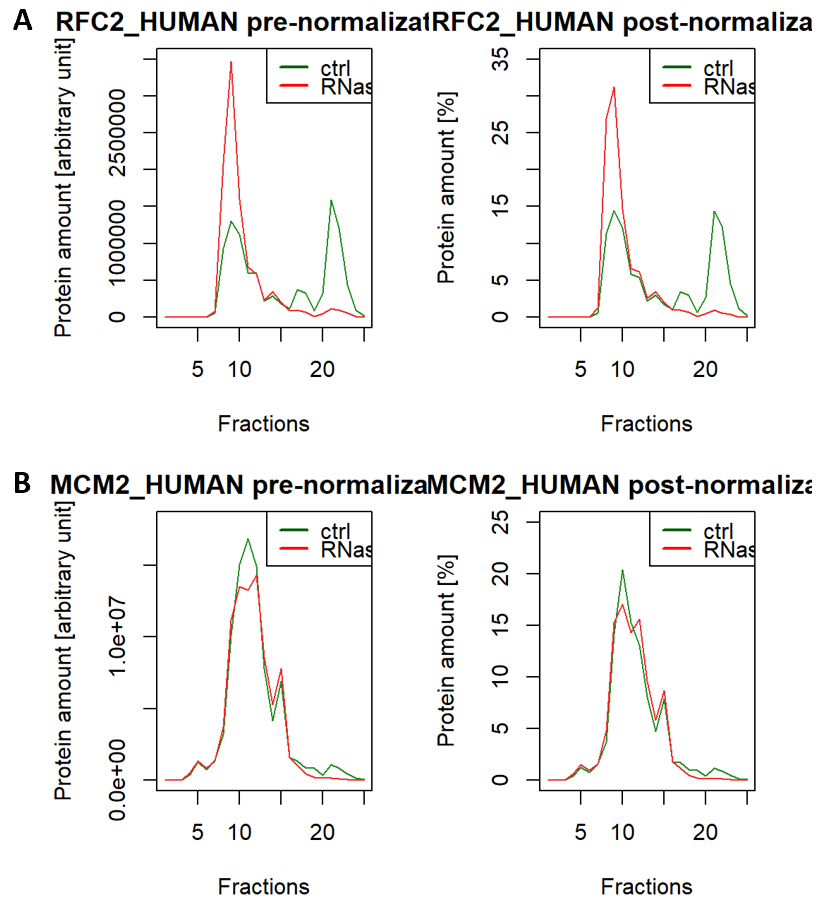
\includegraphics{../../Figure2.PNG}

\textbf{Figure 2: Example of normalization} (A): Comparison of the
sure-shifter RFC2\_HUMAN prior to and post normalization. (B):
Comparison of the non-shifter MCM3\_HUMAN prior to and post
normalization. For both selected proteins the overall distribution trend
is comparable.

\hypertarget{calculation-of-mean-sd-and-shapiro-wilk-test}{%
\subsection{Calculation of mean, sd and Shapiro-Wilk
Test}\label{calculation-of-mean-sd-and-shapiro-wilk-test}}

With the proposed 3\(\sigma\) rule we were able to detect not a single
protein in which at least one replicate was not congruent with a normal
distribution. To verify this result Shapiro-Wilk testwas conducted. Test
concluded that all values obtained for each protein were normally
distributed for both conditions. Therefore they were suitable for
statistical analysis with F-Test and two-tailed unpaired t-test.

\hypertarget{statisitcal-analysis-and-identification-of-potential-rbps-by-analysis-of-x--and-y-shift}{%
\subsection{Statisitcal analysis and Identification of potential RBPs by
analysis of x- and
y-shift}\label{statisitcal-analysis-and-identification-of-potential-rbps-by-analysis-of-x--and-y-shift}}

The obtained x- and y-shift as well as the fraction of the global
maxima, shift direction and y-shift values were stored in a data frame
labeled \emph{abs\_max\_both}.

7081 proteins were tested with F-Test. Only the obtained p-values for
fractions were a global maximum was detected were deemed relevant for
identification of potential RBP candidates. Of 7081 proteins 1196 failed
the test and were excluded from further analysis. 5885 remained.
Quantification of FALSE Results in F-Test resulted that 10 \% of all
analyzed proteins fail F-Test. This means that either one or both
obtained maxima for triplicate measurements vary in their variance in
one treatment compared to the other. Because it seems like some FALSE
F-test results originate from outlier values (see Discussion) and
otherwise we would experience a great exclusion of data, significance
level was set to α = 0.01 instead of the previously usual α = 0.05. With
α = 0.01 closer to 5 \% of data will be excluded based on a FALSE F-test
result. In this compromise some more likely faulty data will still be
excluded while retaining as much data for further analysis as logically
arguable.

Two-tailed unpaired t-test was applied to the remaining 5885 proteins
per fraction ctrl vs RNase. P-Values were checked for significance at
previous determined maxima positions. We identified 2929 potential
shifters.

With the defined cut-off parameters significant y-shift and x-shift
\textgreater{} 1 or significant y-shift and x-shift \textgreater{} 2
these potential shifters were further analysed.

The cut-off \textgreater1 for the x-shift allowed us to identify 513
true RBP with 120 false-positives out of 636 total. Of the 120
false-positives six were identified with cross-recferencing as RBD
proteins. In comparison, the cut-off \textgreater2 for the x-shift
allowed us to identify 398 true RBP with 91 false-positives out of 489
total. Of the 91 false-positives six were identified with
cross-referencing as RBD proteins. The six identified proteins were
identical for both cut-off parameters, and (see Tab.1, data frames
\emph{RBD\_true\_port\_df1} and \emph{RBD\_true\_prot\_df2}).

In both cases, about 80\% of identified RBP were correct when
cross-referenced. Since the \textgreater1 x-shift cut-off did not worsen
this quote but instead delivered more results overall (636 compared to
489), \textgreater1 x-shift cut-off is used for our analysis.

\hypertarget{table.1-amount-of-identified-rbps-true-rbp-quantification-results-after-cross-referencing-obtained-proteins-with-the-additional-data-provided-by-caudron-herger.-tp-true-positive-tn-true-negative-fp-false-positive-fn-false-negative}{%
\subsection{\texorpdfstring{\textbf{Table.1: Amount of identified RBPs:}
True RBP quantification results after cross-referencing obtained
proteins with the additional data provided by Caudron-Herger. TP = True
positive, TN = True negative, FP = False positive, FN = False
negative}{Table.1: Amount of identified RBPs: True RBP quantification results after cross-referencing obtained proteins with the additional data provided by Caudron-Herger. TP = True positive, TN = True negative, FP = False positive, FN = False negative}}\label{table.1-amount-of-identified-rbps-true-rbp-quantification-results-after-cross-referencing-obtained-proteins-with-the-additional-data-provided-by-caudron-herger.-tp-true-positive-tn-true-negative-fp-false-positive-fn-false-negative}}

Criteria \textbar{} x-Shift \textgreater{} 1 \textbar{} x-shift
\textgreater{} 2 \textbar{} Total identified \textbar{} 636 \textbar{}
489 \textbar{} TP \textbar{} 513 \textbar{} 398 \textbar{} FP \textbar{}
120\textbar{} 91 \textbar{} RBD\textbar{} 6 \textbar{} 6\textbar{} ---

\hypertarget{discussion}{%
\section{Discussion}\label{discussion}}

\textbackslash end\{document\}

\end{document}
